%!TEX root = ../main.tex
\section{Results}
\subsection{Rolling correlations}
\begin{figure}[H]
  \caption{Rolling correlations on weekly data - Value factors vs. all factors}
  \label{diag:rolling45}
  \toprule
  \centering
  \begin{minipage}{\textwidth}
  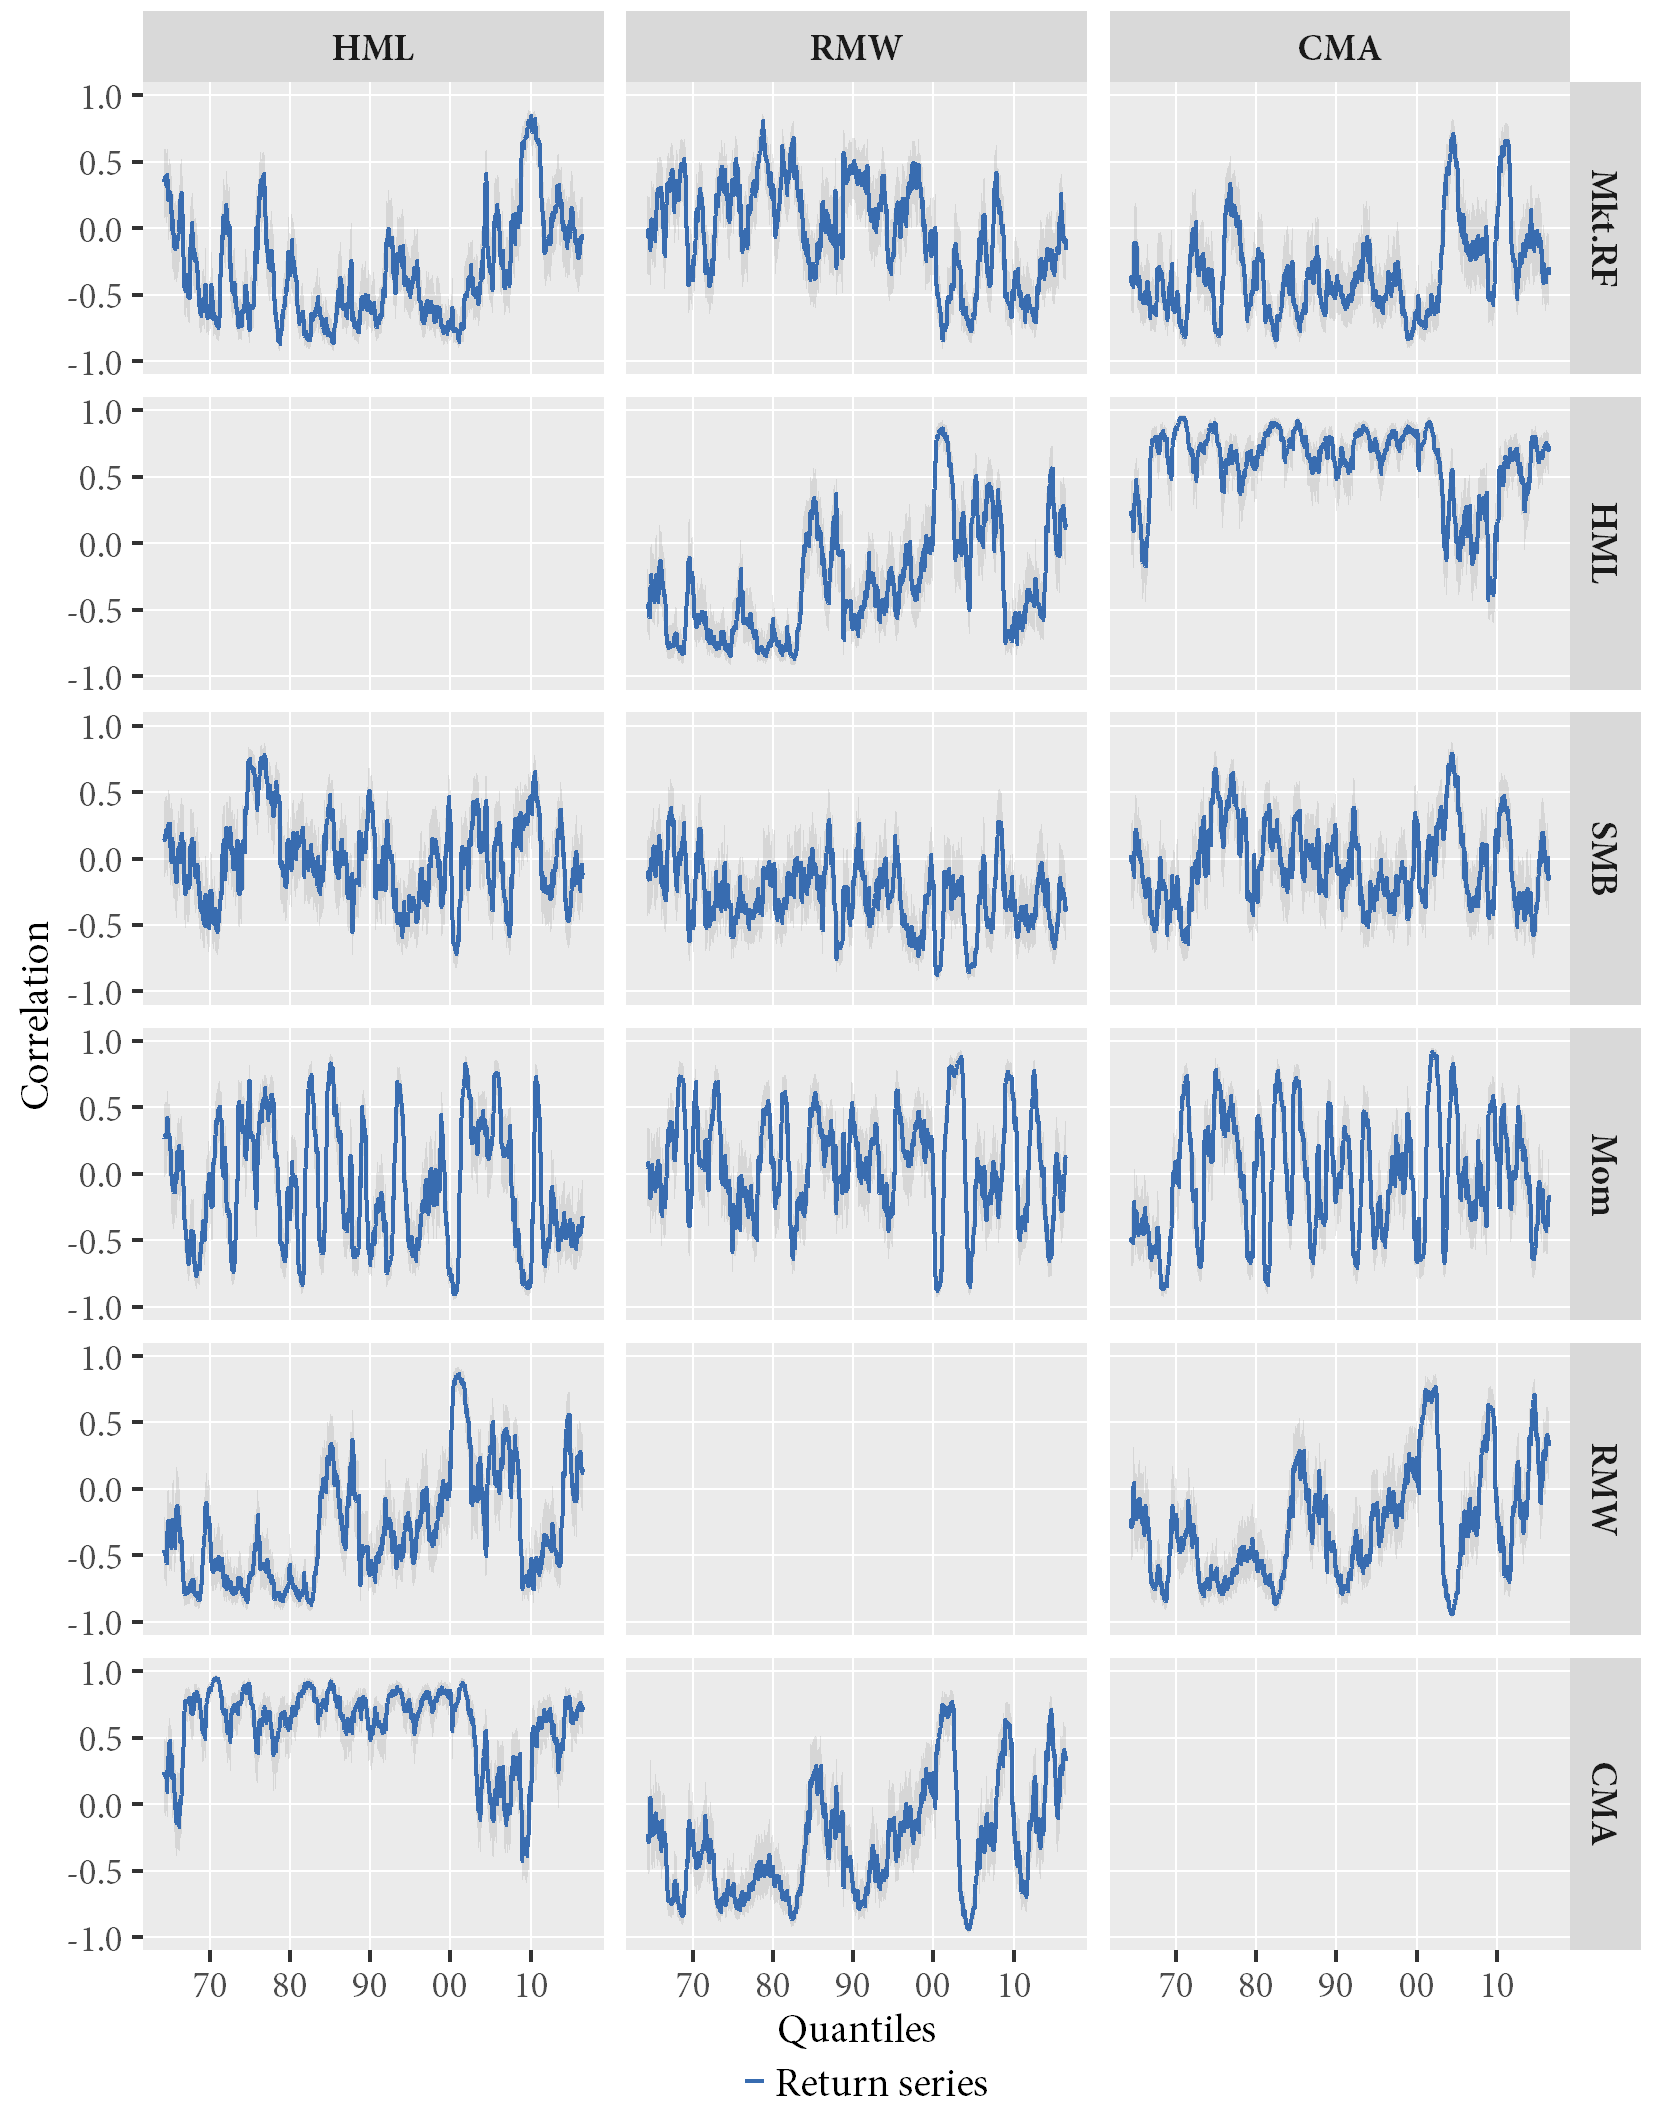
\includegraphics[scale=1]{graphics/rolling45.png}  
  \bottomrule
  \vspace{3mm}
  \footnotesize
  We report rolling 45-week correlations of factor strategy pairs. Return series are weekly log returns. Value factors in columns and all factors in rows. All data 1963-07-05 - 2016-07-01.
  \end{minipage}
\end{figure}
\begin{itemize}
  \item We note that correlations are highly time-varying. Results unchanged if using residuals. Calls for a copula model that can incorporate time variation
\end{itemize}
\subsection{Threshold correlations}
\begin{figure}[H]
  \caption{Threshold correlations on weekly data - Value factors vs. non-value factors}
  \label{diag:thresholdnonvalue}
  \toprule
  \centering
  \begin{minipage}{\textwidth}
  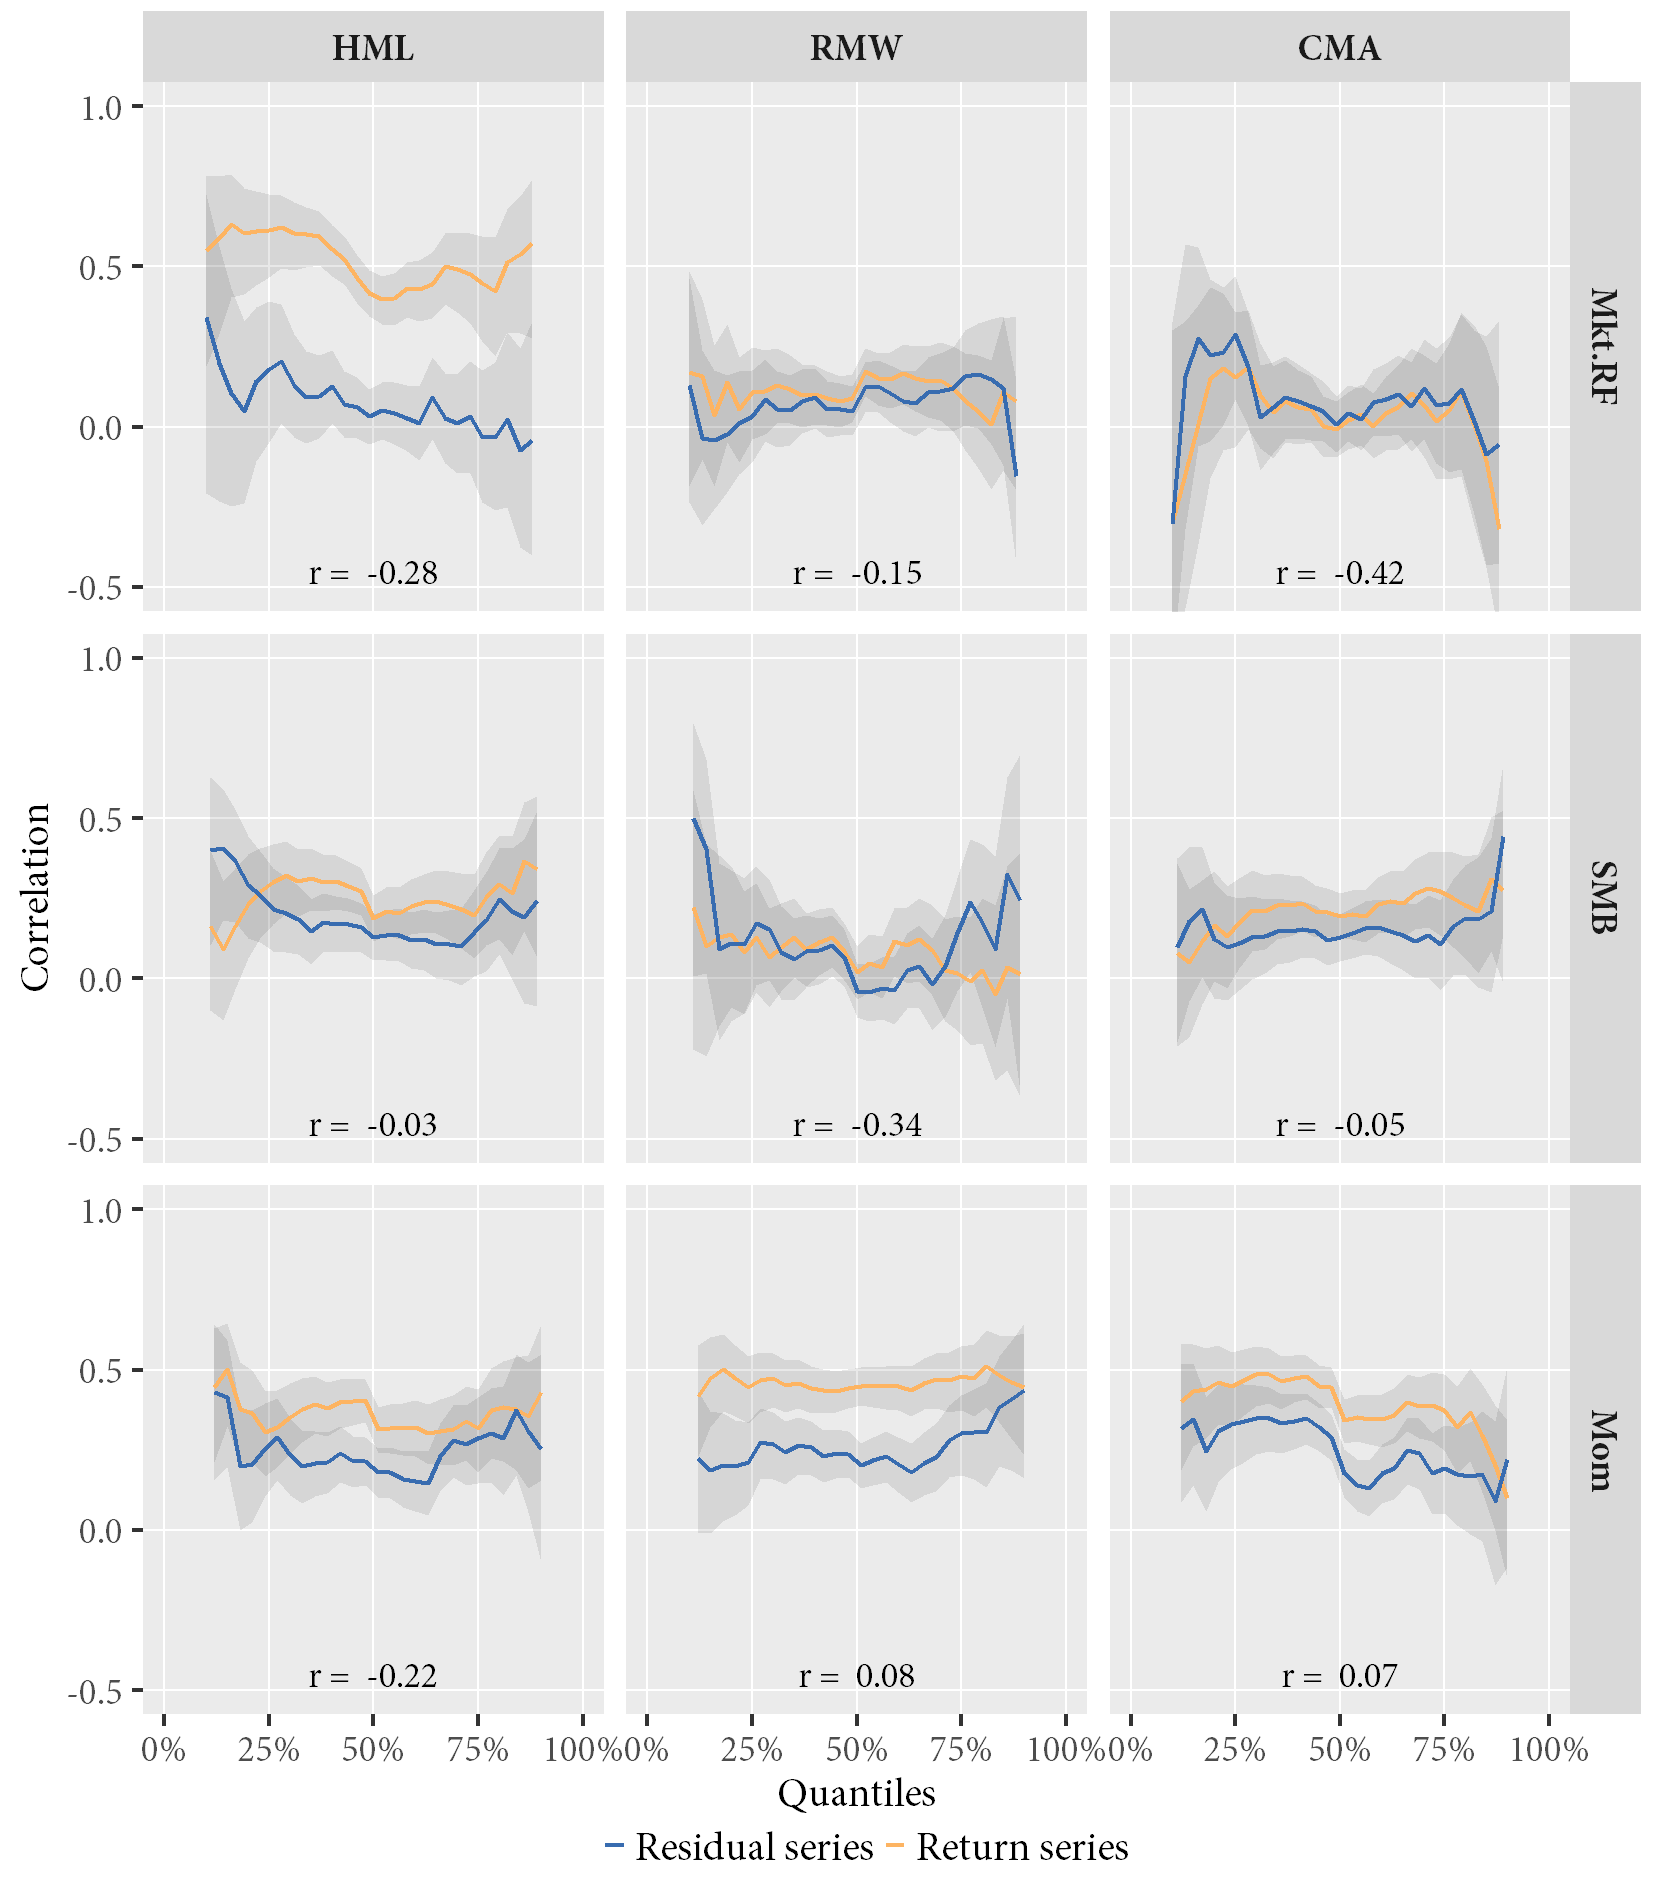
\includegraphics[scale=1]{graphics/threshold_Nonvalue.png}  
  \bottomrule
  \vspace{3mm}
  \footnotesize
  We report threshold correlations of factor strategy pairs. Return series are weekly log returns and residual series are weekly standardized residuals from an ARMA-GJR-GARCH process. Value factors in columns and non-value factors in rows. All data 1963-07-05 - 2016-07-01. Correlations from 10-90\% reported, due to limited data availablility in the tails. Threshold correlations are calculated as: $Corr(r_i, r_j \,|\, r_i < F_i^{-1}(p), r_j < F_j^{-1}(p)) \text{ for } p < 0.5$ and $Corr(r_i, r_j \,|\, r_i \geq F_i^{-1}(p), r_j \geq F_j^{-1}(p)) \text{ for } p \geq 0.5$
  \end{minipage}
\end{figure}
\begin{figure}[H]
  \caption{Threshold correlations on weekly data - Value factors vs. themselves}
  \label{diag:thresholdvalue}
  \toprule
  \centering
  \begin{minipage}{\textwidth}
  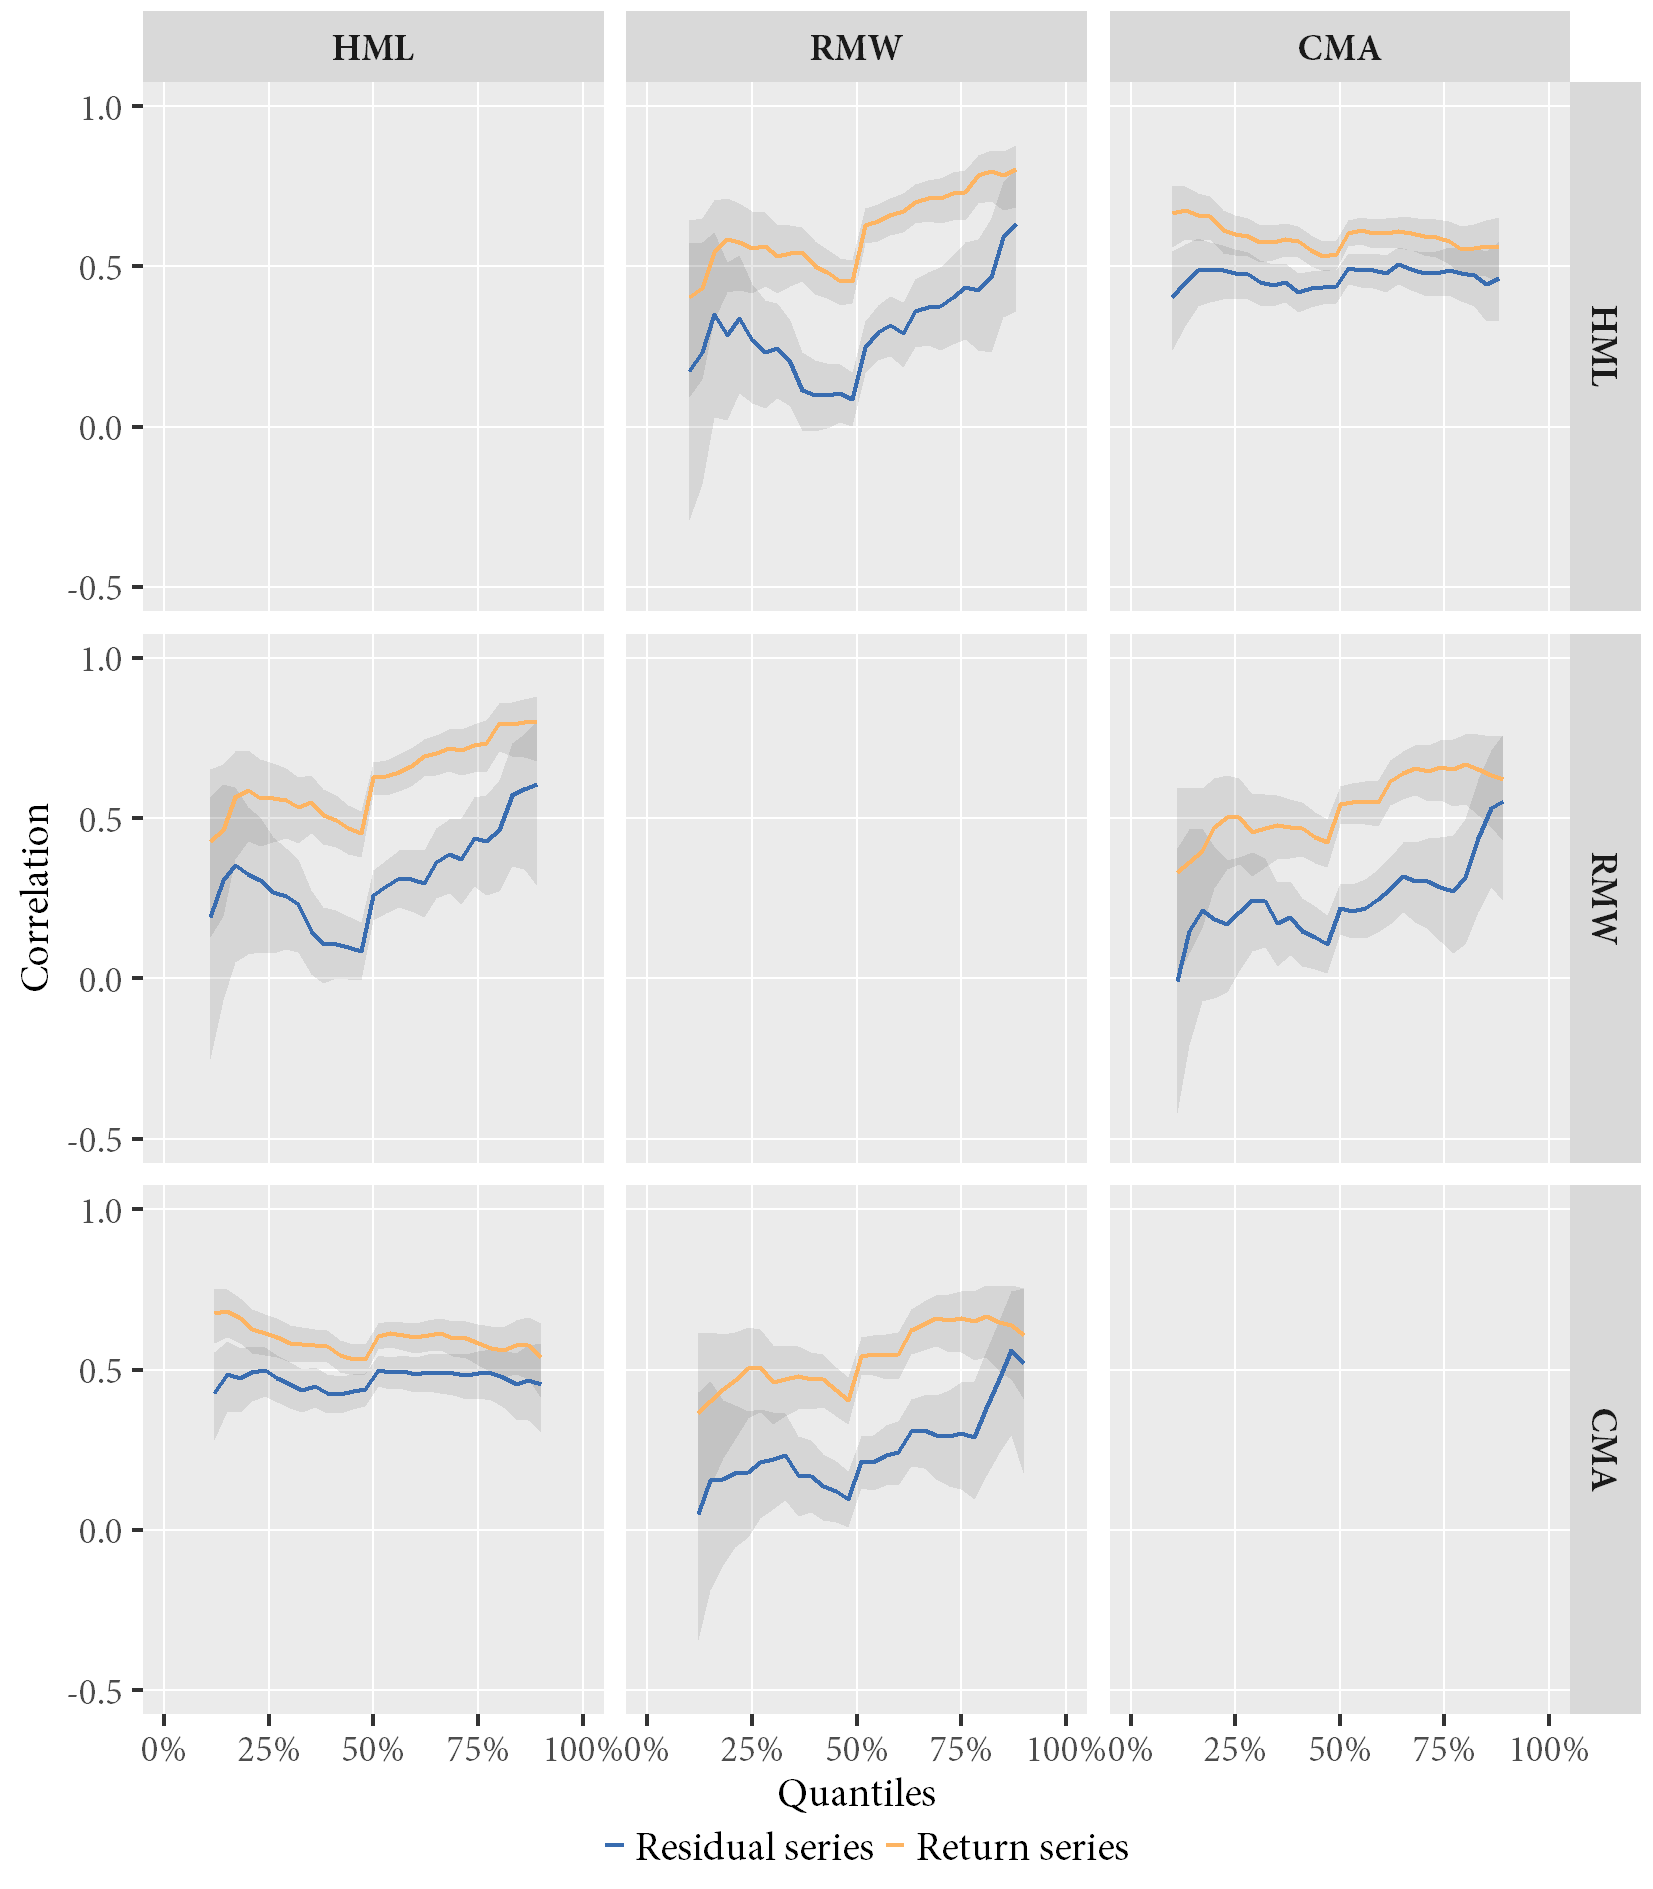
\includegraphics[scale=1]{graphics/threshold_Value.png}  
  \bottomrule
  \vspace{3mm}
  \footnotesize
  We report threshold correlations of factor strategy pairs. Return series are weekly log returns and residual series are weekly standardized residuals from an ARMA-GJR-GARCH process. Value factors in columns and rows. All data 1963-07-05 - 2016-07-01. Correlations from 10-90\% reported, due to limited data availablility in the tails. Threshold correlations are calculated as: $Corr(r_i, r_j \,|\, r_i < F_i^{-1}(p), r_j < F_j^{-1}(p)) \text{ for } p < 0.5$ and $Corr(r_i, r_j \,|\, r_i \geq F_i^{-1}(p), r_j \geq F_j^{-1}(p)) \text{ for } p \geq 0.5$
  \end{minipage}
\end{figure}

\begin{itemize}
  \item There is a marked difference between the threshold correlations before and after applying a GARCH filter. We conclude that a large part of what intially seems as multivariate asymmetry is in fact due to simultaneous ARMA-GARCH effects on the marginal level (reference to market hml graph for example)
  \item Still, there is a lot of tail dependence and asymmetry left. [A Gaussian model with linear correlations approaches zero correlation when the quantile goes to zero and one respectively.] Refernce tail dependency to any graph, reference asymmetry to mkt hml, rmw hml, mom hml, mom cma. 
  \item Market HML is not what you want! others are nicer. supports hypothesis indicative  
\end{itemize}
\subsection{Copula results}
% TABLES NEED TO BE MODIFIED IN THE FOLLOWING WAYS
% 1) Change {tabular} to {tabularx}{\textwidth} and make leftmost column an X column
%     and change top and bottom \hline to \toprule \bottomrule
%
% paste the following at start but before & \multicolumn
%
% \begin{tabularx}{\textwidth}{@{\extracolsep{5pt}} X D{.}{.}{-3} D{.}{.}{-3} D{.}{.}{-3} } 
% \\[-1.8ex] \midrule
% \\[-1.8ex] 
%
% paste the following at end after R2 row but before Note row
% \bottomrule \\[-1.8ex] 
%
% 2) Change the variable names to greeks
% 3) Change specification names if needed
% 4) Change R2 to LLH and add similar lines for Ljung-Box and ARCH-LM
% 5) Add label and caption
% 6) Paste this to get table heading description
% 7) Copy table heading tabularx footnote size text
%
% \begin{tabularx}{\textwidth}{X}
% \\[-1.8ex]\toprule
%\\[-1.8ex] 
% text goes here
% \end{tabularx}
%
% 6) Copy the whole table, only change caption, label, factor/spec labels and (1)-(3) to (4)-(6)
% Table created by stargazer v.5.2 by Marek Hlavac, Harvard University. E-mail: hlavac at fas.harvard.edu
% Date and time: ons, okt 12, 2016 - 12:37:02
% Requires LaTeX packages: dcolumn 
\begin{table}[!htbp] \centering 
  \caption{Copula results: Constant specifications} 
  \label{tab:copula1} 
\begin{tabularx}{\textwidth}{X}
  \\[-1.8ex]\toprule
  \\[-1.8ex] 
  \footnotesize Parameter estimates from constant copula models based on uniform residuals from ARMA-GJR-GARCH models. Stationary bootstrap standard errors in parentheses, following \textcite{PolitisRomano1994}. Copula parameters: $\nu$ is the degree of freedom, $\gamma$ is the vector of skewness parameters, $\alpha, \beta$ are the shock loading and autoregressive loading of the \textit{c}DCC process. All data 1963-07-05 - 2016-07-01. 
\end{tabularx}
\begin{tabularx}{\textwidth}{@{\extracolsep{5pt}} X D{.}{.}{-3} D{.}{.}{-3} D{.}{.}{-3} } 
  \\[-1.8ex]\midrule
  \\[-1.8ex] 
   & \multicolumn{3}{c}{Constant copula models} \\ 
  \cline{2-4} 
  \\[-1.8ex] & \multicolumn{1}{c}{(1)} & \multicolumn{1}{c}{(2)} & \multicolumn{1}{c}{(3)}\\ 
  \\[-1.8ex] & \multicolumn{1}{c}{Gaussian} & \multicolumn{1}{c}{Student-\textit{t}} & \multicolumn{1}{c}{Skewed Student-\textit{t}}\\ 
  \hline \\[-1.8ex] 
 $\nu$ &  & 6.656 & 6.707 \\ 
  &  & () & () \\ 
  & & & \\ 
 $\gamma_{Mkt.RF}$ &  &  & -0.034 \\ 
  &  &  & () \\ 
  & & & \\ 
 $\gamma_{HML}$ &  &  & 0.103 \\ 
  &  &  & () \\ 
  & & & \\ 
 $\gamma_{SMB}$ &  &  & -0.102 \\ 
  &  &  & () \\ 
  & & & \\ 
 $\gamma_{Mom}$ &  &  & -0.183 \\ 
  &  &  & () \\ 
  & & & \\ 
 $\gamma_{RMW}$ &  &  & 0.019 \\ 
  &  &  & () \\ 
  & & & \\ 
 $\gamma_{CMA}$ &  &  & 0.086 \\ 
  &  &  & () \\ 
  & & & \\ 
 $\alpha$ & 0 & 0 & 0 \\ 
  &  &  &  \\ 
  & & & \\ 
 $\beta$ & 0 & 0 & 0 \\ 
  &  &  &  \\ 
  & & & \\ 
\hline \\[-1.8ex] 
Observations & \multicolumn{1}{c}{2,766} & \multicolumn{1}{c}{2,766} & \multicolumn{1}{c}{2,766} \\ 
LLH & \multicolumn{1}{c}{1,170} & \multicolumn{1}{c}{1,549} & \multicolumn{1}{c}{1,564} \\ 
Correlation $(Q)$ persistence $(\alpha+\beta)$ & \multicolumn{1}{c}{0} & \multicolumn{1}{c}{0} & \multicolumn{1}{c}{0} \\ 
\bottomrule \\[-1.8ex] 
\textit{Note:}  & \multicolumn{3}{c}{$^{*}$p$<$0.1; $^{**}$p$<$0.05; $^{***}$p$<$0.01} \\ 
\end{tabularx} 
\end{table} 
% Table created by stargazer v.5.2 by Marek Hlavac, Harvard University. E-mail: hlavac at fas.harvard.edu
% Date and time: ons, okt 12, 2016 - 12:37:02
% Requires LaTeX packages: dcolumn 
\begin{table}[!htbp] \centering 
  \caption{Copula results: \textit{c}DCC specifications} 
  \label{tab:copula2} 
\begin{tabularx}{\textwidth}{X}
\\[-1.8ex]\toprule
\\[-1.8ex] 
\footnotesize Parameter estimates from dynamic copula models based on uniform residuals from ARMA-GJR-GARCH models. Stationary bootstrap standard errors in parentheses, following \textcite{PolitisRomano1994}. Copula parameters: $\nu$ is the degree of freedom, $\gamma$ is the vector of skewness parameters, $\alpha, \beta$ are the shock loading and autoregressive loading of the \textit{c}DCC process. All data 1963-07-05 - 2016-07-01. 
\end{tabularx}
\begin{tabularx}{\textwidth}{@{\extracolsep{5pt}} X D{.}{.}{-3} D{.}{.}{-3} D{.}{.}{-3} } 
\\[-1.8ex]\midrule
\\[-1.8ex] 
 & \multicolumn{3}{c}{Dynamic copula models} \\ 
\cline{2-4} 
\\[-1.8ex] & \multicolumn{1}{c}{(4)} & \multicolumn{1}{c}{(5)} & \multicolumn{1}{c}{(6)}\\ 
\\[-1.8ex] & \multicolumn{1}{c}{Gaussian} & \multicolumn{1}{c}{Student-\textit{t}} & \multicolumn{1}{c}{Skewed Student-\textit{t}}\\ 
\hline \\[-1.8ex] 
 $\nu$ &  & 11.831 & 11.803 \\ 
  &  & () & () \\ 
  & & & \\ 
 $\gamma_{Mkt.RF}$ &  &  & -0.055 \\ 
  &  &  & () \\ 
  & & & \\ 
 $\gamma_{HML}$ &  &  & 0.071 \\ 
  &  &  & () \\ 
  & & & \\ 
 $\gamma_{SMB}$ &  &  & -0.170 \\ 
  &  &  & () \\ 
  & & & \\ 
 $\gamma_{Mom}$ &  &  & -0.125 \\ 
  &  &  & () \\ 
  & & & \\ 
 $\gamma_{RMW}$ &  &  & 0.095 \\ 
  &  &  & () \\ 
  & & & \\ 
 $\gamma_{CMA}$ &  &  & 0.022 \\ 
  &  &  & () \\ 
  & & & \\ 
 $\alpha$ & 0.066 & 0.068 & 0.068 \\ 
  & () & () & () \\ 
  & & & \\ 
 $\beta$ & 0.915 & 0.913 & 0.913 \\ 
  & () & () & () \\ 
  & & & \\ 
\hline \\[-1.8ex] 
Observations & \multicolumn{1}{c}{2,766} & \multicolumn{1}{c}{2,766} & \multicolumn{1}{c}{2,766} \\ 
LLH & \multicolumn{1}{c}{2,791} & \multicolumn{1}{c}{2,975} & \multicolumn{1}{c}{2,984} \\ 
Correlation $(Q)$ persistence $(\alpha+\beta)$ & \multicolumn{1}{c}{0.980} & \multicolumn{1}{c}{0.981} & \multicolumn{1}{c}{0.981} \\ 
\bottomrule \\[-1.8ex] 
\textit{Note:}  & \multicolumn{3}{c}{$^{*}$p$<$0.1; $^{**}$p$<$0.05; $^{***}$p$<$0.01} \\ 
\end{tabularx} 
\end{table} 
\begin{itemize}
  \item Large step up in LLH from constant to dynamic copula. Consistent with fact that correlations vary over time. Reference to graph
  \item Asymmetry parameters generally significantly estimated, but the change in LLH is not as great as for the change from the normal specification
  \item Comment on variance non-persistence
  \item Vuong test conclusion
\end{itemize}

\subsection{Conditional diversification benefit}
\begin{figure}[H]
  \caption{Conditional diversification benefit}
  \label{diag:cdb1}
  \toprule
  \centering
  \begin{minipage}{\textwidth}
  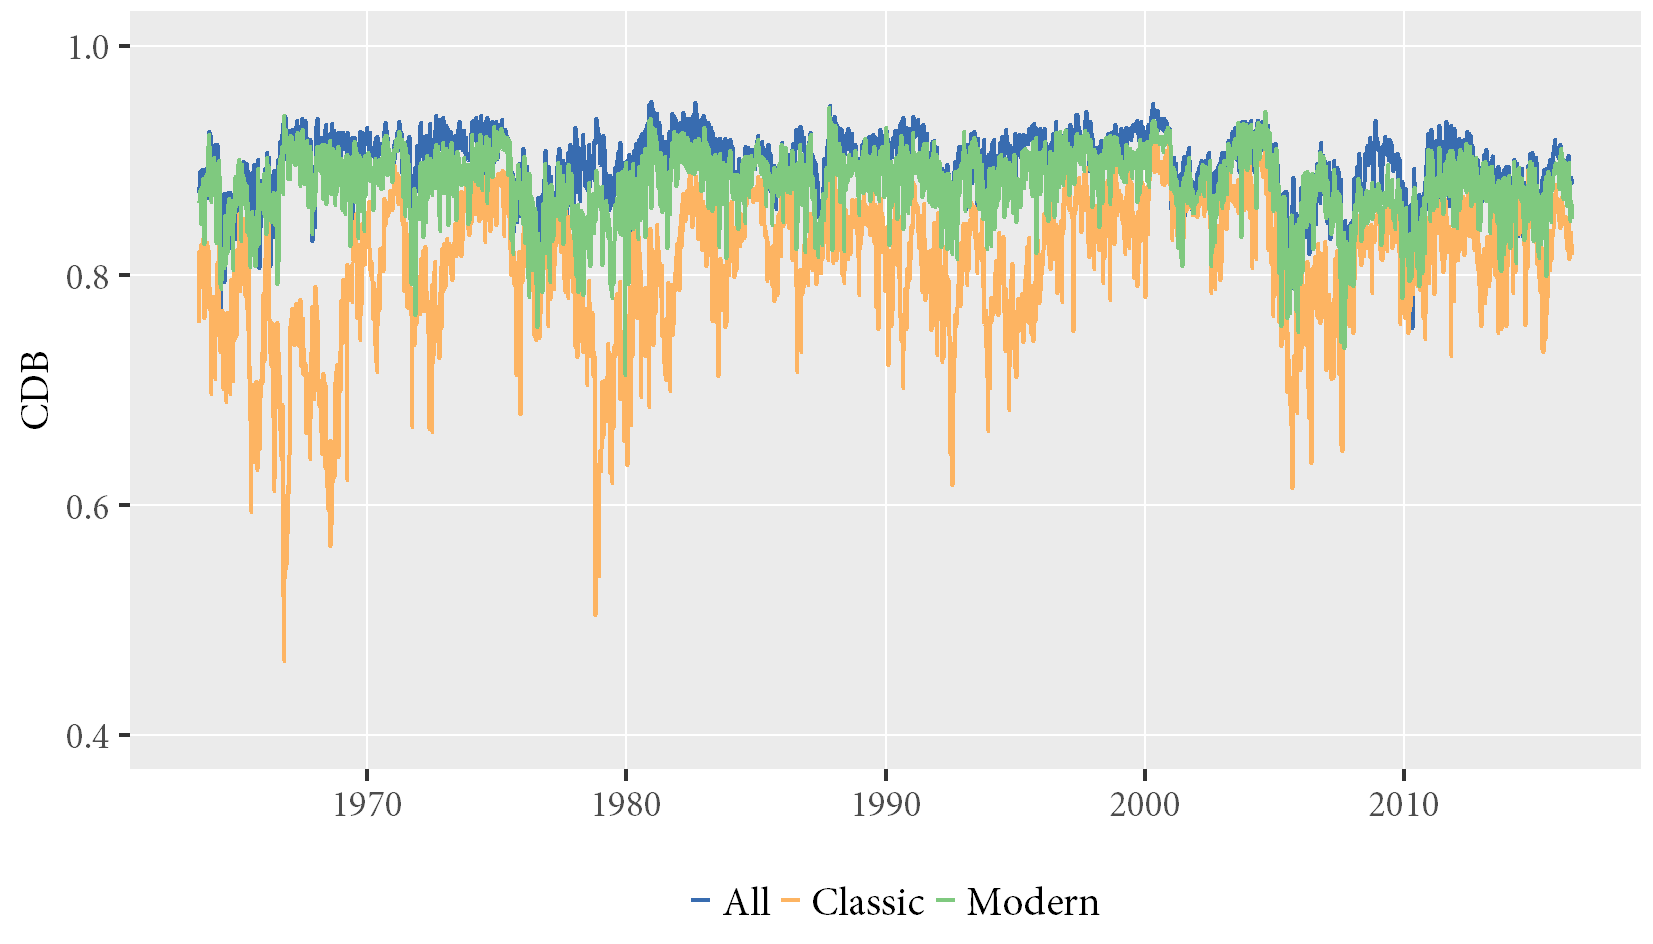
\includegraphics[scale=1]{graphics/CDB_dynamic_ghskt.png}  
  \bottomrule
  \vspace{3mm}
  \footnotesize
  We report conditional diversification benefit of three asset universes: All (including $Mkt.RF$, $HML$, $SMB$, $Mom$, $RMW$, $CMA$), Classic (All excluding $RMW$, $CMA$), and Modern (All excluding $HML$). A value closer to one indicates greater diversification benefit and a value of zero indicates no diversification benefit. All data 1963-07-05 - 2016-07-01, using simulations from the copula model.
  \end{minipage}
\end{figure}
\begin{itemize}
  \item Modern value is better diversified than classic value. Introducing $RMW$ and $CMA$ to the factor universe makes expected shortfall closer to the theoretical upper bound (smaller losses).
  \item It seems to be in times of non-crisis that classic value underperforms more - note that the $CDB$ is relatively more clustered around crises of 1973-1976, 1999-2001, 2008-2010.
\end{itemize}